\section{The Replication Study}
\label{sec:replication-replication}

Our key goal is to investigate whether the conclusions of Pinto \etal generalize to different flakiness scenarios, viz., (1) a time-sensitive prediction use case where flakiness information about past tests are used to predict flakiness in future (new) tests, (2) flakiness prediction in different programming languages, (3) the use of different sets of features involving both test code and code under test. Each of these scenarios gives rise to a research question that we answer in our study. In all scenarios, we use the model presented in the original study that gave the best performance. The model is based on a bag of words and a Random Forest of 100 trees i.e., the model which gave the best results in the original study. Our replication package containing code, models and datasets is available online\footnote{\url{https://github.com/serval-uni-lu/FlakyVocabularyReplication}}.

\subsection{Research Questions}
We aim at answering the following research questions:
\begin{itemize}[label={}]
\item \textbf{\textsc{RQ1:}} \emph{How  well  do  vocabulary-based  models  identify flaky  tests  when  using  a  time-sensitive validation?}
\item \textbf{\textsc{RQ2:}} \emph{How  well  do  vocabulary-based  models  identify flaky tests in other programming languages?}
\item \textbf{\textsc{RQ3:}} \emph{Is the vocabulary of Code Under Test useful for flakiness prediction?}
\end{itemize}

\subsection{RQ1: Time-Sensitive Validation}
In the real world, one can picture different usages for a flaky test prediction model. 
For instance, in Continuous Integration (CI) environments where new changes (commits) making some tests fail are typically rejected, developers can ignore those failing tests that are likely to be flaky and isolate them for further investigation.

In another setting, the prediction model can also come as an IDE plugin hinting at tests that use keywords related to flakiness.

These scenarios illustrate the importance of the temporality of tests and code, as the model can be trained only on flaky tests detected previously to predict new occurrences.
Moreover, the fact that the vocabulary of code changes as new commits are introduced makes it challenging for models trained on older data to predict flakiness in future code versions that are temporarily distant.

The model can also be limited to flaky tests detected in one project, e.g., when the vocabulary linked to flakiness can differ from one project to another. 
Indeed, as reported in the literature~\cite{Luo2014,Lam2019RootCausing}, different sources of flakiness exist such as concurrency issues, usage of date/time, I/O actions, API or network calls, etc. 
Thus, based on the project, the flakiness sources can differ and the vocabulary associated with it varies accordingly.

For all these reasons, we propose a novel, intra-project, time-sensitive setup for validating flakiness prediction models.
This setup evaluates a model on its ability to predict new flaky tests with data that is assumed to be known from the past of the project.

To compare this setup with the one from Pinto \etal, we rely on the DeFlaker dataset, which was also used in the original study.
For each project, we select tests that were found flaky at any revision of the change history to form the Flaky Tests set $FT$. 
DeFlaker does not provide explicit information about tests that did not flake, as the tool can not guarantee that a test that did not fail (yet) is not flaky. 
We define Non Flaky Tests $NFT$ as tests that were not found as flaky in any revision, that is, $NFT = T_{Total} - FT$.

Figure~\ref{time-validation} explains how FT and NFT are selected in our time-sensitive validation. We split our dataset in order to have 80\% of the FT from earlier revisions for our training set and 20\% of the FT from "future" revisions for our test set. 

We select the $NFT$ from the revision where the last $FT_{train}$ are selected for the training set and from the last revision where $FT_{test}$ are selected for the test set.

To assess the impact of this new setup on model performance, we compare it with a classical setup where the model is trained and tested with flaky tests regardless of their observation date (i.e., the setup followed by Pinto \etal).
In such setup, all flaky and non-flaky tests are grouped without accounting for their observation date. 
Then, the groups are randomly split into training and test sets following an 80/20 ratio. 

\begin{figure}
\centering
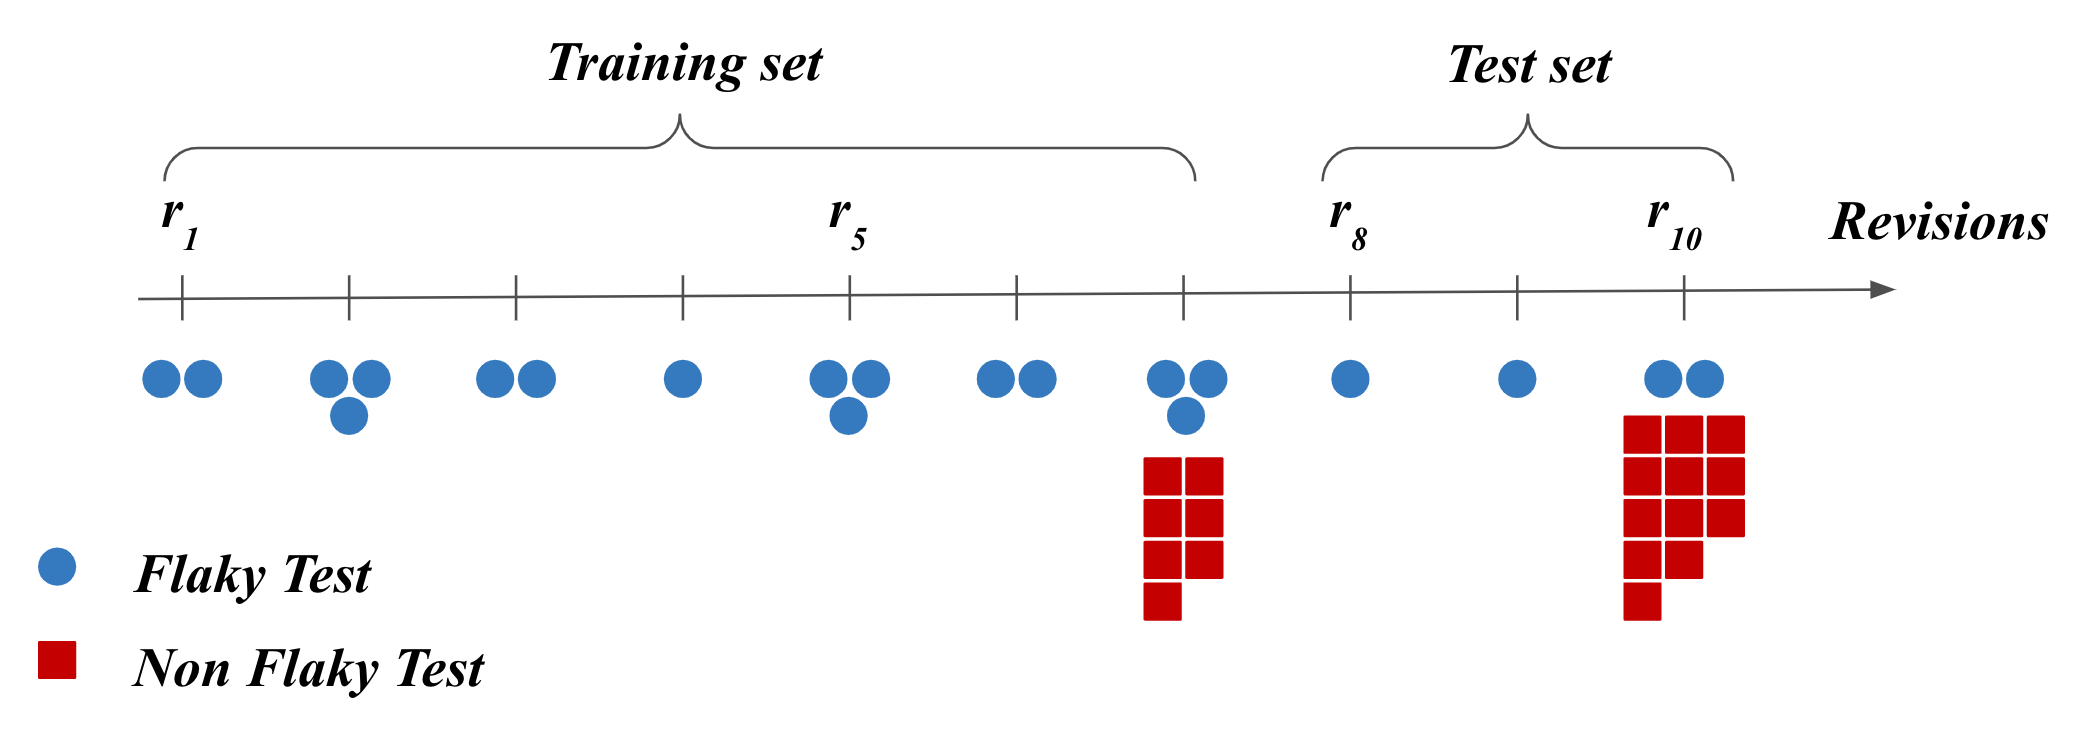
\includegraphics[width=0.8\textwidth]{figures/replication/fig1.png}
\caption{Time-sensitive validation}
\label{time-validation}
\end{figure}

To perform this comparison, we selected six projects from the DeFlaker dataset based on their numbers of flaky tests. 
These projects have at least 30 flaky tests, which we consider as a minimum necessary for training and testing a model. 
Table ~\ref{javaInfo} presents these projects with their numbers of flaky and non-flaky tests.
We also present the dates of the first and last flaky tests identified in these projects.
We split this dataset according to the two validation setups, then we build our prediction model, train it and contrast the results of both setups.

\begin{table}
\centering
\caption{Details about the Java projects used in our study}
\label{javaInfo}
 \begin{tabular}{l|r r r r r} 
 \toprule
 \textbf{Project} & \textbf{Earliest revision} & \textbf{Latest revision} &\textbf{ \#FT} & \textbf{\#NFT} \\ [0.25ex]
 \midrule
 achilles & 2015-10-30 & 2016-09-05 & 51 & 392 \\
 hbase & 2010-05-17 & 2010-06-21 & 98 & 120\\
 okhttp & 2014-03-06 & 2015-01-30 & 102 & 1178\\
 oozie & 2013-03-20 & 2013-05-31 & 1039 & 44 \\
 oryx & 2015-01-06 & 2015-02-27 & 38 & 286 \\ 
 togglz & 2016-01-23 & 2016-06-17 & 20 & 256 \\ 
 \bottomrule
\end{tabular}
\end{table}



\subsection{RQ2: Generalisation to other Programming Languages}
\subsubsection{Predicting flaky tests in Python}
Another goal of our study is to evaluate the generalisability of the original study to other programming languages.
For this purpose, we propose to assess the performance of flakiness prediction models on Python projects. 
We chose Python because it is the most popular language used in modern projects and it is commonly used for machine learning, web development, game development, and many other applications.

Python comes with its set of testing frameworks. 
We focus our study on Pytest\cite{pytestdocumentation}. Pytest is the equivalent of Junit for Python and enables developers to write tests for their programs. It is one of the main testing frameworks used in the open-source community and in the industry.
Pytest comes with its lot of features and plugins. Especially, a specific module to handle flaky tests can be used with Pytest: flaky\footnote{\url{https://pypi.org/project/flaky/}}.  
This module allows developers to annotate tests as flaky to automatically rerun them in case of failure. 
The developer can also configure the maximum amount of reruns to attempt and the minimum number of passes required. 
This annotation can be added to a test function or directly to the test class, giving its property to all of its tests. 
Figure~\ref{flaky-example} shows an example of a test marked as \emph{@flaky} taken from the Typed\_python project\footnote{\url{https://github.com/APrioriInvestments/typed\_python}}.

\begin{figure}[ht]
\centering
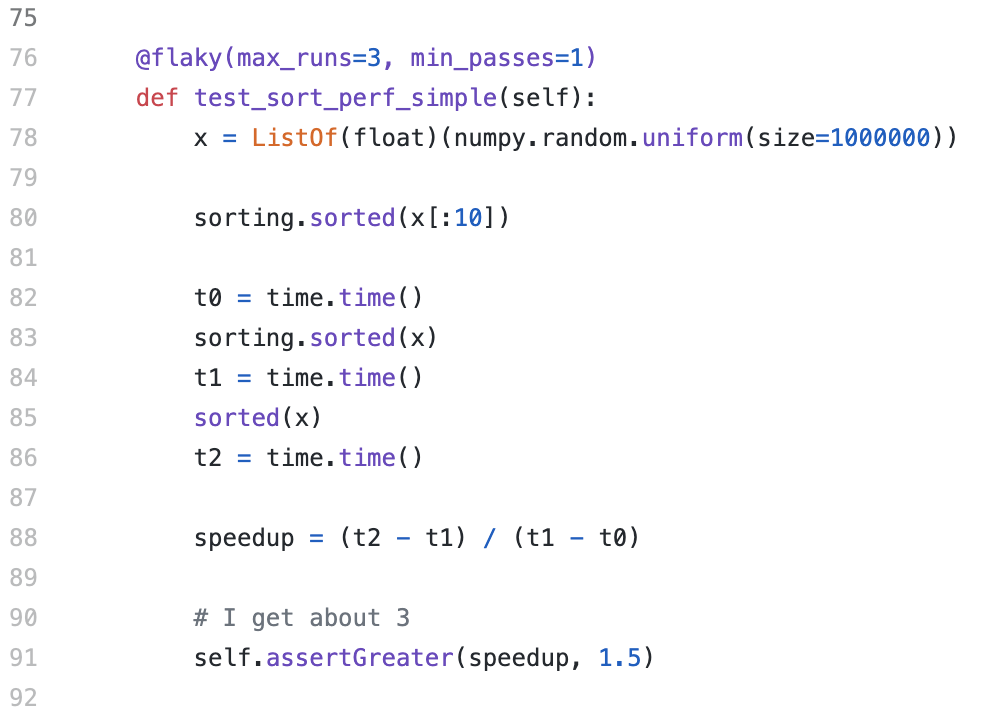
\includegraphics[width=0.8\textwidth]{figures/replication/flakyExample.png}
\caption{Example of a test labelled @flaky}
\label{flaky-example}
\end{figure}

We mined GitHub using the source-graph API\footnote{\url{https://sourcegraph.com/search}}, searching for Python projects containing the annotation \emph{@flaky}. 
This process yielded 110 projects with a total of 1,304 tests marked as flaky. 
Similarly to our first experimentation, we only select projects in which we have enough flaky tests to train and test a model, \ie 30 flaky tests.
This results in a dataset of 9 projects and 837 tests marked by developers as flaky.
Table ~\ref{pythonInfo} shows these projects with their number of flaky and non-flaky tests. 
Compared to the Java dataset, we were able to obtain more projects with more flaky tests for our study.
To the best of our knowledge, this is the first dataset of flaky tests in Python.

\begin{table}
\centering
\caption{Python projects used in our study}
\label{pythonInfo}
 \begin{tabular}{l|r r r r r} 
 \toprule
 \textbf{Project} & \textbf{SHA} & \textbf{\#FT }& \textbf{\#NFT}\\ [0.25ex]
 \midrule
 bokeh & ddc22b8 & 100 & 2505 \\
 cassandra-dtest & 8cb6bd2 & 72 & 4221 \\
 celery & 0833a27 & 54 & 2890 \\
 jira & 7fa3a45 & 131 & 59 \\
 pipenv & 8e64873 & 32 & 1612 \\
 python-amazon & 84c16f5 & 35 & 15 \\
 python-telegram-bot & 8e7c0d6 & 186 & 1382 \\
 spyder & 413c994 & 173 & 1086 \\
 typed-python & 96e7ebd & 54 & 6034 \\ 
 \bottomrule
\end{tabular}
\end{table}

It is worth noting that in this research question, we evaluate the performance of the model to predict flaky tests in a single revision. Therefore, we reuse the typical 80/20 dataset split as followed by Pinto \etal.  
That is, we are rather focusing on confirming that the approach works as well in Python and that a model can learn features differentiating tests labelled as \emph{@flaky} from the ones that are not. 
To extract these features, we use a bag of words representation of the test, as in Java. 
We also carefully remove the \emph{@flaky} annotations, as keeping it in the vocabulary would bias our model towards recognising this annotation rather than the code vocabulary.


\subsubsection{Predicting manifest flaky tests}
We perform further analysis in Python to assess the usefulness of a vocabulary-based model. 
Our objective is to evaluate the ability of a model to identify \textit{manifest} flaky tests based on training with tests labelled as flaky by developers. 
We consider as manifest flaky, every test for which we are able to observe non-deterministic behaviour dynamically.
This means that the test fails and passes at least once after several reruns.
To identify these manifest flaky tests, we reran 200 to 300 times the test suite of the three projects Bokeh, Celery and Python-telegram-bot. 
We run the test suites on a Mac machine with a 2,4 GHz 8-Core i9 processor and 32Gb of RAM.
The results of these reruns are presented in the table ~\ref{manifestStudy}.
The column \#@flaky shows the number of tests labelled as flaky in each project.
\begin{table}
\centering
\caption{Classifier performance for Python projects with manifest flaky tests}
\label{manifestStudy}
 \begin{tabular}{l|r r r r r} 
 \toprule
 \textbf{Project} & \textbf{\#reruns} & \textbf{\#@flaky} & \textbf{\#manifest FT}\\ [0.25ex]
 \midrule
 bokeh & 200 & 100 & 1 \\
 celery & 300 & 54 & 2 \\
 python-telegram-bot & 300 & 186 & 20 \\ 
 \bottomrule
\end{tabular}
\end{table}

We observe that despite the high number of reruns (800), only 23 tests have a flaky behaviour. This outcome is not surprising as flaky tests are, by nature, difficult to reproduce. To assess the model performance in detecting manifest flaky tests, we focus on the only project that has a reasonable amount of manifest flaky tests, namely Python-telegram-bot. We use the 20 manifest flaky tests found during our reruns as a test set, completed by 20 randomly selected tests that are not labelled as flaky. For the training set, we use the flaky and non-flaky tests minus the tests present in the test set. 

\subsection{RQ3: Extended Set of Features}
So far, the flakiness prediction is only based on features taken from the test code. 
However, flaky tests can be due to infrastructure or environmental issues (\eg lack of available resources in the CI, service or network unavailable, etc), to the test itself (\eg usage of dates, randomness, order dependency, etc), or to the CUT (\eg non-determinism, concurrency, etc). 
Notably, Luo~\etal~\cite{Luo2014} showed that 24\% of the fixes for flaky tests were applied to the CUT and that among them, 94\% fixed a bug in the CUT. 
Hence, it can be judicious to consider information from the CUT in flakiness prediction models. We propose to extend the original study by including the vocabulary of the CUT in test representation.

The main issue when considering the CUT is that computing the code coverage of each test during each revision would bring significant overheads. 
Besides, retrieving the exact code coverage dynamically goes against the goal of static prediction, which is to reduce dynamic costs.
To avoid this overhead, we propose a lightweight approach that relies on Information Retrieval (IR) to estimate the CUT. 

IR techniques have been used to solve different software engineering problems~\cite{Saha2014,Palomba2018,Azizi2018}. 
IR aims at quickly and automatically retrieving relevant information among a set of documents based on keywords taken from a user query. 
In our case, the query is the tokens of a test and the set of documents is the set of all functions (or methods) defined in the project. 
Our hypothesis is that functions from the CUT of a test are likely to use similar keywords (\ie variable names, API calls, etc) as the test. We are then looking for the most similar functions to our test function. To do so, we use a cosine similarity between a test case and a function from the CUT. Cosine similarity is defined with: 
\[cosSimilarity = \cos (Tc, Func) = \frac{Tc \cdot Func}{|Tc| |Func|}\]
where $Tc$ is the vector representing the test code and $Func$ is the vector representing the function code.
The result of a cosine similarity ranges from -1, meaning that the query - our test case - is completely different from the document - our function - to 1, where the query is perfectly similar to the document. 
In our case, we select the top three most similar functions for each test. 

\begin{algorithm}
\SetAlgoLined
\textbf{Inputs:}\\
Test[]\\
Function[]\\
\textbf{Outputs:}\\
TestWithCUT[]\\
\textbf{Procedure} \emph{CUT\_SELECTION(Test[], Function[])}\\
 \ForEach{ test T $ \in $ Test[]}{
   similarityMeasures[]\\
   Tvector = transform(T)\\
   \ForEach{function F $ \in $ Function[]}{
     fit($T+F$)\\
     Fvector = transform(F)\\
     cosTF = cosSimilarity(Tvector, Fvector)\\
     similarityMeasures.Append(cosTF)\\
   }
  similarityMeasures.Sort()\\
  similarityMeasures.Slice(0, 2)\\
  T.append(similarityMeasures)\\
  TestWithCUT.append(T)\\
 }
 \textbf{return} TestWithCUT[]
 \caption{Cost effective retrieval of the CUT}
 \label{algo}
\end{algorithm}

Algorithm~\ref{algo} describes the process of associating the CUT to each test. 
In order to compute the cosine similarity between the test and a function, we use the Text tokenisation utility class from the Keras library\footnote{\url{https://keras.io/api/preprocessing/text/}}. 
We first fit the \emph{Tokeniser} with the vocabulary from all tests and functions. 
Then, we transform the text of test and function bodies by creating a vector for each one of them of a length equal to the size of the vocabulary.
In this vector, each element represents the number of times a word appears in the body. 
After extracting the vectors, we compute the cosine similarity between the current test and all functions and store results. 
We finally filter to only keep functions that have a high score, \ie that they are the closest to the test. 
The body representation of the selected functions is used as a new set of features for the flakiness prediction model.